%%%%%%%%%%%%%%%%%%%%%%%%%%%%%%%%%%%%%%%%%
% CU Boulder Physics Lab Writeup One Column
% LaTeX Template
% Version 1.0 (2022-10-05)
%
% This template has been downloaded from:
% http://www.LaTeXTemplates.com
%
% Original author:
% Mathias Legrand (legrand.mathias@gmail.com) titled Stylish Article 
% With extensive modifications by:
% Vel (vel@latextemplates.com)
% Further modifications for CU Boulder Physics by:
% Kristopher Bunker (kristopher.bunker@colorado.edu)
%
% License:
% CC BY-NC-SA 3.0 (http://creativecommons.org/licenses/by-nc-sa/3.0/)
%
%%%%%%%%%%%%%%%%%%%%%%%%%%%%%%%%%%%%%%%%%

%----------------------------------------------------------------------------------------
%	PACKAGES AND OTHER DOCUMENT CONFIGURATIONS
%----------------------------------------------------------------------------------------

\documentclass[10pt]{PhysLab1C} % Document font size

\usepackage[english]{babel} % Specify a different language here - english by default

%----------------------------------------------------------------------------------------
%	COLUMNS
%----------------------------------------------------------------------------------------

\setlength{\columnsep}{0.55cm} % Distance between the two columns of text
\setlength{\fboxrule}{0.75pt} % Width of the border around the abstract

%----------------------------------------------------------------------------------------
%	COLORS
%----------------------------------------------------------------------------------------

\definecolor{color1}{RGB}{0,0,90} % Color of the article title and sections
\definecolor{color2}{RGB}{0,20,20} % Color of the boxes behind the abstract and headings


%----------------------------------------------------------------------------------------
%	HYPERLINKS
%----------------------------------------------------------------------------------------

\usepackage{hyperref} % Required for hyperlinks

\hypersetup{
	hidelinks,
	colorlinks,
	breaklinks=true,
	urlcolor=color2,
	citecolor=color1,
	linkcolor=color1,
	bookmarksopen=false,
	pdftitle={Title},
	pdfauthor={Author},
}

%----------------------------------------------------------------------------------------
%	LAB AND COURSE INFORMATION
%----------------------------------------------------------------------------------------

\CourseInfo{Electronics for the Physical Sciences \vert ~ \textbf{PHYS 3330}} %
\Department{\copyright \ Department of Physics \vert ~ \textbf{University of Colorado Boulder} \ \vert ~ \textbf{\today}} %
\Copyright{\today} %
\LabTitle{Operational Amplifiers (OP-Amps) I} % Lab Title

%----------------------------------------------------------------------------------------
%	ABSTRACT
%----------------------------------------------------------------------------------------

\Abstract{\textbf{Lab 4:} Introduction to op-amps and the non-inverting amplifier.}

%----------------------------------------------------------------------------------------

\begin{document}

\maketitle % Output the title and abstract box

%\tableofcontents % Output the contents section

\thispagestyle{firstpage} % Removes page numbering from the first page

%----------------------------------------------------------------------------------------
%	ARTICLE CONTENTS
%----------------------------------------------------------------------------------------

\section{Goals}

In this lab, you will characterize the gain and frequency dependence of
op-amp circuits, one of the most useful components in electronics. You
will also measure input and output impedances of these circuits. The
op-amp is the most important building block of analog electronics. As
op-amps are made out of transistors, most textbooks discuss transistors
first, followed by op-amps. We choose the opposite order as we are not
particularly interested in how op-amps are constructed but rather how to
use them in circuits and the principles of op-amps operation are
actually simpler than for transistors.

Proficiency with new equipment:

\begin{itemize}
\item
  Op-amps: Non-inverting amplifier with unity gain (voltage follower)
  and finite gain
\end{itemize}

Proficiency with new analysis and plotting techniques:

\begin{itemize}
\item
  Bode plots
\end{itemize}

Modeling the physical system:

\begin{itemize}
\item
  Frequency dependence of op-amp circuits
\item
  Input and output impedances of op-amp circuits
\end{itemize}

%------------------------------------------------

\section{Definitions}

\textbf{Closed-loop gain, $G$} - gain of the \emph{op-amp circuit} at all
frequencies with feedback applied

\textbf{Low frequency gain, $G_{0}$} - gain of the
\emph{op-amp circuit} at DC (f = 0 Hz)

\textbf{Open-loop gain, $A$} - gain of the \emph{op-amp itself} at all
frequencies with no feedback applied

\textbf{DC gain, $A_{0}$} - gain of the \emph{op-amp itself}
at DC (f = 0 Hz) with no feedback applied

$\mathbf{f_0}$ - 3 dB frequency for an \emph{op-amp
itself} with no feedback

$\mathbf{f_B}$ - 3 dB frequency for an \emph{op-amp
circuit} with feedback applied

$\mathbf{f_T}$- unity gain frequency, frequency
where the open loop gain $A$ is equal to one

%------------------------------------------------

\section{General Purpose of OP-Amps}


One of the main purposes of an amplifier is to increase the voltage
level of a signal while preserving as accurately as possible the
original waveform. In the physical sciences, transducers are used to
convert basic physical quantities into electric signals, as shown in
Figure \ref{lab-measurement}. An amplifier is usually needed to raise the small transducer
voltage ($\mu V$ to $mV$) to a useful level ($mV$ to $V$).

\begin{figure}[h]\centering
    
\includegraphics{tmp.png}
    \caption{Typical laboratory measurement system}
    \label{lab-measurement}
\end{figure}


Measuring and recording equipment typically requires input signals of $10~
mV$ to $10~ V$. To meet such needs, a typical laboratory amplifier might
have the following characteristics:

\begin{enumerate}
\def\labelenumi{\arabic{enumi}.}
\item
  Predictable and stable gain. The magnitude of the gain is equal to the
  ratio of the output signal amplitude to the input signal amplitude.
\item
  Linear amplitude response, so that the output signal is directly
  proportional to the input signal.
\item
  According to the application, the frequency dependence of the gain
  might be a constant independent of frequency up to the highest
  frequency component in the input signal (wideband amplifier), or a
  sharply tuned resonance response if a particular frequency must be
  picked out.
\item
  High input impedance and low output impedance are usually desirable.
  These characteristics minimize changes of gain when the amplifier is
  connected to the input transducer and to other instruments at the
  output.
\item
  Low noise is usually important. Every amplifier adds some random noise
  to the signals it processes, and this noise often limits the
  sensitivity of an experiment.
\end{enumerate}

Commercial laboratory amplifiers are readily available, but a
general-purpose amplifier is expensive (\textgreater{}\$1000), and most
of its features might be unneeded in a given application. Often, it is
preferable to design your own circuit using a cheap (\textless\$1)
op-amp chip. Op-amps have many other circuit applications. They can be
used to make comparators, filters, limiters, rectifiers, oscillators,
integrators, and other devices. We will build some of these circuits in
later labs.

%------------------------------------------------

\section{OP-Amp Basics}


Two basic op-amp circuit configurations, the non-inverting amplifier and
the inverting amplifier, are shown in Figures \ref{non-invert} and \ref{invert}, respectively.
Both circuits use \emph{\textbf{negative feedback}}, which means that a
portion of the output signal is sent back to the negative input of the
op-amp through the feedback resistor RF. The op-amp itself has very high
gain, but relatively poor gain stability and linearity. When negative
feedback is used, the circuit gain is greatly reduced, but it becomes
very stable. Also, linearity is improved, and the output impedance
decreases.

\begin{figure}[h]
%\centering
\hspace{1cm}
\begin{subfigure}[t]{0.3\textwidth}
%\centering
\begin{circuitikz}[american voltages]
    \draw (0,0) node[anchor = east]{$V_{in}$} to[short, o-] ++(1,0) 
    node[op amp, noinv input up, anchor=+](OA){\texttt{}} 
    (OA.-) -- ++(-.5,0) to ++(0,-1.5) to ++(3.5,0) coordinate(FB) 
    to [R, l_=$R$] ++(2,0) node[ground]{} 
    (OA.out) to (OA.out -| FB) to [R=$R_F$, *-*] ++(0,-2) to (FB)
    (OA.out) to [short, -o] ++(2,0) node[anchor = west]{$V_{out}$}
    ;
\end{circuitikz}
 \caption{Non-inverting amplifier}
 \label{non-invert}
 \end{subfigure}
 \hspace{3cm}%
 \begin{subfigure}[t]{0.3\textwidth}
% \centering
\begin{circuitikz}[american voltages]
    \draw (0,0) node[op amp, anchor=-](OA){\texttt{}} 
    (OA.+) -- ++((-.5,0) to ++(0,-.5) node[ground]{}
    (OA.-) -- ++((-.5,0) to ++(0,1) coordinate(FC) to [R, l_=$R$, *-] ++(-2,0)
    to [short, -o] ++(0,0) node[anchor = east]{$V_{in}$}
    (FC) to [R=$R_F$] ++(2,0) to [short] ++(1,0) coordinate(FD)
    (FD) to [short, -*] (OA.out -| FD){}
    (OA.out) to [short, -o] ++(1.5,0) node[anchor = west]{$V_{out}$}
    ;
\end{circuitikz}
 \caption{Inverting amplifier}
 \label{invert}
 \end{subfigure}
 \caption{OP-Amp circuits}
 \end{figure}


Both configurations are widely used because they have different
advantages. Besides the fact that the second circuit inverts the signal,
the main differences are that the first circuit has much higher input
impedance, while the second has lower distortion because both inputs
remain very close to ground. In this lab, we will be focusing on the
first-type, non-inverting.



The gain or transfer function, $A$, of the \textbf{op-amp alone} is given
by

\[A\equiv\frac{V_{out}}{V_{in}^+-V_{in}^-}\]

where the denominator is the difference between the voltages applied to
the + and - inputs. We use the symbol \(G\) for the gain of the complete
amplifier with feedback: \(G = V_{out}/V_{in}\). This gain depends on
the resistor divider ratio

\[B = \frac{R}{R + R_{F}}\]

If we assume an ideal situation where \(A = \infty\), that the op-amp input
impedance is infinite, and that the output impedance is zero, then the
behavior of these circuits can be understood using the simple "Golden
Rules":

\begin{enumerate}
\def\labelenumi{\arabic{enumi}.}
\item
  \textbf{The voltage difference between the inputs is zero. ("voltage
  rule")}
\item
  \textbf{No current flows into (or out of) each input. ("current
  rule")}
\end{enumerate}

The ``Golden Rule'' analysis is very important and is always the first
step is designing op-amp circuits, so be sure you understand it before
you read the material below, where we consider the effect of finite
values of $A$.


\subsection{Non-inverting amplifier}


The basic formula for the low frequency gain of non-inverting amplifiers
is derived in Steck Section 7.3.3. Using just the Golden rules, which
assumes \(A\gg 1\), the gain is given by

\[G_{0} = \frac{V_{out}}{V_{in}} =\frac{R+R_F}{R} = 1 + \frac{R_{F}}{R}\]

Equations for the input and output impedance of the entire circuit are
derived in H\&H Section 4.26. The results are

\[R_{i}^{'} = R_{i}(1 + AB)\]
\[R_{o}^{'} = R_{o}/(1 + AB)\]

where \(R_i\) and \(R_o\) are the input and output impedances of the
\emph{op-amp alone}, while the primed symbols refer to the whole
amplifier with feedback. These impedances will be improved from the
values for the bare op-amp if \(A\cdot B\) is large.

The above formulas are still correct when \(A\) and/or \(B\) depend on
frequency. \(B\) will be frequency independent if we have a resistive
feedback network (in other cases that use complex impedance it may not
be), but \(A\) always varies with frequency. For most op-amps, including
the LF356, the open loop gain varies with frequency like an RC low-pass
filter:

\[A(f)=\frac{A_0}{1+j\frac{f}{f_0}}\]

The 3dB frequency, \(f_0\), is usually very low, around 10 Hz. Data
sheets do not usually give \(f_0\) directly; instead they give the DC
gain, \(A_0\), and the unity gain frequency \(f_T\), which is the
frequency where the magnitude of the open loop gain A is equal to one.
The relation between \(A_0\), \(f_0\), and \(f_T\) is

\[f_{T} = A_{0}f_{0}\]

The frequency dependence of the closed loop gain $G$ is then given by:

\[G(f)=\frac{G_0}{1+j\frac{f}{f_B}}\]

The frequency response of the amplifier with feedback is therefore also
the same as for an RC low-pass filter.

We can now derive an example of a very important general rule connecting
the gain and bandwidth of feedback amplifiers. Multiplying the low
frequency gain \(G_0\) by the 3 dB bandwidth \(f_B\) gives

\[A_0 f_0=G_0 f_B = f_T\]

In words, this very important formula says that the gain-bandwidth
product \(G_0f_B\) equals the unity gain frequency \(f_T\). Thus if an
op-amp has a unity gain frequency \(f_T\) of 1 MHz, it can be used to
make a non-inverting amplifier with a gain of one and a bandwidth of 1
MHz, or with a gain of 10 and a bandwidth of 100 kHz, \emph{etc.} We
will consider what this means for the transfer function as a function of
frequency on a Bode plot.

%------------------------------------------------

\section{Useful Readings}


\begin{enumerate}
\item
  \href{https://atomoptics-nas.uoregon.edu/~dsteck/teaching/electronics/electronics-notes.pdf}{Steck} Sections 7.1, 7.2, 7.3.1, 7.3.3
  
\item
  Fischer-Cripps Sections 12.2 -- 12.15
\item
  Horowitz and Hill 2\textsuperscript{nd} Ed., Chapter 4
\end{enumerate}

%------------------------------------------------

\section{Prelab}

Answer the following questions using Mathematica for the plots. You can
use either Mathematica for the rest of the questions as well or do them
by hand. \textbf{Make sure to have the Mathematica notebook for your lab
section as well.}

\subsection{Properties of and op-amp}

The first step in using a new component is to look up its basic
characteristics. Find the following specs using the data sheet for the
op-amp you will use in the lab for the rest of the semester. Data for
the LF356 op-amp (same as LF156) are given at the National Semiconductor
web site and found in Canvas in the Datasheets section.

\begin{enumerate}
\item
  Unity gain frequency, \(f_T\) (same as GBW in tables)
\item
  DC voltage gain, \(A_0\) (same as \(A_{VOL}\) in tables)
  \textbf{(convert to a unitless quantity)}
\item
  Maximum output voltage (same as \(V_O\) in tables)
\item
  Maximum output positive current at 0 V for a supply voltage of ±15 V
  (look for a graph)
\item
  Input resistance, \(R_i\)
\end{enumerate}

\subsection{Non-inverting amplifier}


\begin{enumerate}
\item
  Calculate the values of the low frequency gain \(G_0\) and bandwidth
  \(f_B\) for the non-inverting amplifier in Figure \ref{non-invert} for the following
  two circuits you will build in lab.

  \begin{enumerate}
  \item
    \(R_F = 10 ~k\Omega\) and \(R = 100 ~\Omega\)
  \item
    \(R_F = 0\) and \(R = \infty\) (this is a voltage follower)
  \end{enumerate}
\item
  Predict the output voltage, \(V_{out}\), for the non-inverting amp
  with \(R_F = 10 ~k\Omega\) and \(R = 100 ~\Omega\) with ±15 V power supply rails
  when

  \begin{enumerate}
  \item
    \(V_{in} = 1~ mVDC \)
  \item
    \(V_{in} = 1 ~V\) (you may find your answer to 6.1.3 useful)
  \end{enumerate}
\item
  Create Bode plots for the open loop gain and the two closed loop gains
  from 6.2.1 on the same graph using Mathematica (label each curve and
  cover at least 1--10\textsuperscript{8} Hz).
\item
  Estimate the input impedance of the complete amplifier circuit
  (\(R_i^{'}\)) with \(R_F = 10 ~k\Omega\) and \(R = 100 ~\Omega\) for 1 kHz sine
  waves.
\item
  Estimate the output impedance of the complete amplifier circuit
  (\(R_o^{'}\)) with \(R_F = 10 ~k\Omega\) and \(R = 100 ~\Omega\) for 1 kHz sine
  waves. The nominal output impedance of the LF356 alone is $40~\Omega$. To
  obtain the circuit output impedance at 1 kHz, one can use this value
  and determine \(R_o^{'}\) using the formula given above. Alternatively, one
  can read off the value from the top left plot on page 7 of the
  datasheet. This shows the output impedance for an inverting amplifier
  (which has the same output impedance as a non-inverting amplifier) as
  a function of frequency for gains of \(A_v=~1,~10,~100\).
\end{enumerate}

\subsection{Lab activities}


\begin{enumerate}
\item
  Read through all of the lab steps and identify the step that you think
  will be the most challenging.
\item
  List at least one question you have about the lab activity.
\end{enumerate}

%------------------------------------------------

\section{Setting Up a Basic OP-Amp Circuit}


All op-amp circuits start out by making the basic power connections.
Op-amps are active components, which means they need external power to
function, unlike passive components such as resistors and capacitors.


\begin{figure}[h]
 \centering
 \begin{circuitikz}[american voltages]
    \draw (0, 0) node[op amp] (opamp) {};
    \draw (opamp.-) node[above right]{2} node[anchor = east]{$V_-$};
    \draw (opamp.+) node[above right]{3} node[anchor = east]{$V_+$};
    \draw (opamp.out) node [above left]{6} node[anchor = west]{$V_{out}$};
    \draw (opamp.up) node[above right]{7} to (-.08,1.25) node[anchor = south]{$+15~V$};
    \draw (opamp.down) node[below right]{4} to (-0.08,-1.25) node[anchor = north]{$-15~V$};
    \path (2.5,0.75) node[dipchip, anchor=pin 1, num pins=8]{LF356};
 \end{circuitikz}
 \caption{LF356 schematic and pin-out.}
  \label{lf356}
\end{figure}

\begin{figure}
    \centering
    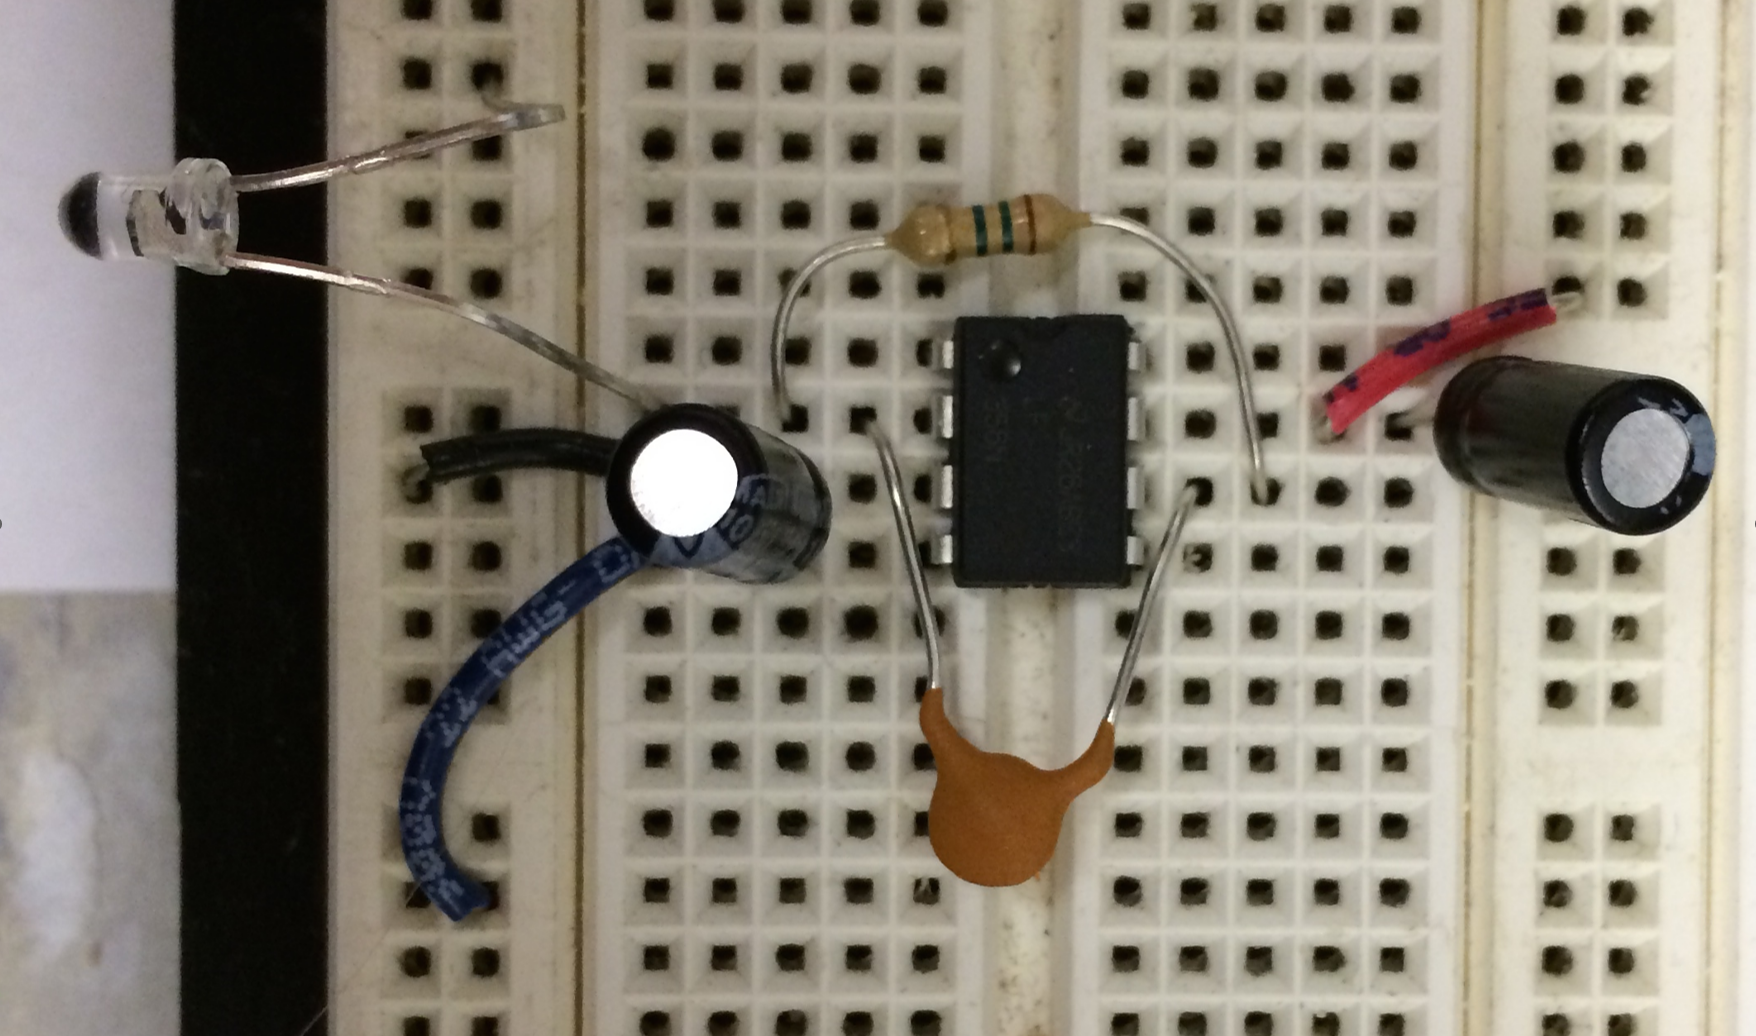
\includegraphics[width=10cm]{lab4fig/pb-example.png}
    \caption{Good placement of op-amp and bypass capacitors on a
protoboard. Note that short wires are used for all connections.}
    \label{pb}
\end{figure}

\subsection{Op-amp setup}


\begin{enumerate}
\item
  This experiment will use both +15 V and --15 V to power the LF356
  op-amp. \textcolor{red}{Make sure you \textbf{unplug} the DC supplies while wiring
  your op-amp (you may find it useful to plug them into their own power
  strip). Everyone makes mistakes in wiring-up circuits. You should
  always check your circuit over before applying power.} Figure \ref{lf356} shows a
  pin-out for the LF356 chip. Familiarize yourself with the layout. The
  following procedure will help you wire up a circuit accurately:

  \begin{enumerate}
  \item
    Draw a complete schematic in your lab notebook, including all ground
    and power connections, and all IC pin numbers. Try to layout your
    prototype so the parts are arranged in the same way as on the
    schematic, as far as possible.
  \item
    Measure all resistor values before putting them in the circuit. Make
    sure you are using the correct capacitors. Some capacitors indicate
    the capacitance directly, but small capacitors usually just have a
    number where 10 = 10 pF, 102 = 10x10\textsuperscript{2} pF = 1 nF,
    103 = 10x10\textsuperscript{3} = 10 nF, 104 =
    10x10\textsuperscript{4} pF = 100 nF. Also, see the important note
    below about polarized capacitors.
  \item
    Adhere to a color code for wires. For example:

    \begin{itemize}
    \item
      \textcolor{OliveGreen}{0V (ground) Green}
    \item
      \textcolor{red}{+15V Red}
    \item
      \textcolor{blue}{-15V Blue}
    \end{itemize}
  \end{enumerate}
\item
  The op-amp chip sits across a groove in the prototyping board (see Figure \ref{pb}). Before inserting a chip, ensure the pins are straight (using a
  needle-nose pliers or something similar). After insertion, check
  visually that no pin is broken or bent under the chip. To remove the
  chip, use a small screwdriver in the groove to pry it out.
\item
  You will have less trouble with spontaneous oscillations if the
  circuit layout is neat and compact, in particular the feedback path
  should be as short as possible to reduce unwanted capacitive coupling
  (see Figure \ref{pb}). Also, wire around the chip rather than over it.
\item
  To help prevent spontaneous oscillations due to unintended coupling
  via the power supplies, use bypass capacitors to filter the power
  supply lines. A bypass capacitor between each power supply lead and
  ground will provide a miniature current ``reservoir'' that can quickly
  supply current when needed. This capacitor is normally in the range
  1--10 µF. \textcolor{red}{Compact capacitors in this range are usually
  \emph{\textbf{polarized}}, meaning that one terminal must always be
  positive relative to the other. If you put a polarized capacitor in
  backwards, it will burn out.} You will probably hear a pop and smell
  something foul. Please don't do this. The negative side should have an
  arrow on the capacitor. Also, the positive side should have a longer
  lead but this is not a good identification method as the leads can
  (and should) be cut. Bypass capacitors should be placed close to the
  op-amp pins. If you are connecting the +15 V supply to ground, the
  negative capacitor lead is connected to ground and the positive lead
  is connected to +15 V. If you are connecting the --15 V supply to
  ground, the negative capacitor lead is connected to --15 V and the
  positive lead is connected to ground.
\end{enumerate}

\subsection{Testing the op-amp}


\begin{enumerate}
\item
  You can save yourself some frustration by testing your op-amp chips to
  make sure they are not burned out. Connect the op-amp as a
  grounded-input \emph{\textbf{voltage follower}} with the (positive)
  input grounded (see Figure \ref{voltage-follower-gnd}). What is the predicted voltage on pins 2,
  3, 4, 6 and 7 using the Golden Rule model? Measure and record the
  measured voltages on these pins. If your predictions do not match your
  measurements check your connections to the chip to find the problem.
  Make sure your predictions match your measurements before going on.
\item
  If you find you have a bad chip, throw it in the trash and grab
  another. (In case you are wondering, the LF356 costs about 50 cents.)
\end{enumerate}

\begin{figure}[h]
    \centering
\begin{circuitikz}[american voltages]
    \draw (0,0) node[op amp, anchor=-](OA){\texttt{}} 
    (OA.+) -- ++((-.5,0) to ++(0,-.5) node[ground]{}
    (OA.down) to [short, -o] ++(0,-1) node[anchor = north]{$-15~V$}
    (OA.down) to [short, -*] ++(0,-.5) to [C] ++(2,0) node[ground]{}
    (OA.up) to [short, -o] ++(0,1) node[anchor = south]{$+15~V$}
    (OA.up) to [short, -*] ++(0,.5) to [C] ++(2,0) node[ground]{}
    (OA.out) -- ++(1.25,0) coordinate(FC) to [short, -o] ++(1,0) node[anchor = west]{$V_{out}$}
    (OA.-) -- ++(-.5,0) to ++(0,2) to ++(4.5,0) to [short,-*] ++(0,-2.5)
    ;
\end{circuitikz}
    \caption{Schematic of a voltage follower with the input grounded.}
    \label{voltage-follower-gnd}
\end{figure}


%------------------------------------------------

\section{Voltage Follower}


A voltage follower is the simplest version of a non-inverting amplifier.
The voltage follower has no voltage gain (G\textsubscript{0}=1), but it
lets you convert a signal with high impedance (i.e. very little current)
to a much lower impedance output for driving loads. The voltage follower
is also often called a unity gain buffer.

\begin{figure}[h]
    \centering
\begin{circuitikz}[american voltages]
    \draw (0,0) node[op amp, anchor=-](OA){\texttt{}} 
    (OA.+) to [short,-o] ++(-.5,0) node[anchor = east]{$V_{in}$}
    (OA.down) to [short, -o] ++(0,-1) node[anchor = north]{$-15~V$}
    (OA.down) to [short, -*] ++(0,-.5) to [C] ++(2,0) node[ground]{}
    (OA.up) to [short, -o] ++(0,1) node[anchor = south]{$+15~V$}
    (OA.up) to [short, -*] ++(0,.5) to [C] ++(2,0) node[ground]{}
    (OA.out) -- ++(1.25,0) coordinate(FC) to [short, -o] ++(1,0) node[anchor = west]{$V_{out}$}
    (OA.-) -- ++(-.5,0) to ++(0,2) to ++(4.5,0) to [short,-*] ++(0,-2.5)
    ;
\end{circuitikz}
    \caption{Voltage follower.}
    \label{voltage-follower}
\end{figure}

\subsection{Low frequency gain and frequency dependence of the gain}


\begin{enumerate}
\def\labelenumi{\arabic{enumi}.}
\item
  The voltage follower circuit is nearly the same as the test circuit,
  except that now a signal enters the positive input (Figure \ref{voltage-follower}). The basic
  test and measurement setup is shown in Figure \ref{op-amp-test}.
\item
  Use the function generator to measure the low frequency gain. What
  frequency should you use to test the low frequency gain (i.e., what
  frequency should the signal be below)? Consider the gain-bandwidth
  product for a unity gain amplifier. What is the gain-bandwidth product
  for this circuit? How did you find the value? What is the predicted
  gain for the frequency you chose? Measure the low frequency gain
  \(G_0\) by measuring \(V_{in}\) and \(V_{out}\) using the scope. Do
  your measurements agree with your predictions?
\item
  Now vary the frequency and look for deviation from the performance of
  an ideal follower model. The measurement at high frequency will depend
  on many details of your setup and you are unlikely to find a simple RC
  filter type falloff. Using the 10X scope-probe, measure the gain at
  every decade in frequency from 10 MHz down to 10 Hz, with (as usual) a
  few extra points anywhere things are starting to change. Do you find
  any deviation from unity gain? HINT: Be sure that the output amplitude
  is below the level affected by the slew rate For help, see H\&H p.
  192. Plot the low and high frequency data and predicted behavior on
  your Bode plot from your lab prep. Do you find a simple fall-off as
  suggested by the theory for the ideal follower (\(f_T=f_B\))? If so,
  find the 3 dB frequency. How does your measured 3 dB frequency compare
  to what is expected from the op-amp datasheet?
\item
  If you observed ideal behavior, you\textquotesingle re lucky! At
  frequencies above a few MHz, the simple model of the frequency
  response of the op-amp is not accurate. Once you are in this frequency
  range, many physical details of your circuit and breadboard can have
  large effects in the circuit (see notes in 7.1.4 above). You could
  model these effects, but a better procedure to follow is to modify the
  physical setup. Building reliable circuits at these frequencies
  typically requires careful attention to grounding and minimization of
  capacitive and inductive coupling between circuit elements and to
  ground. Printed circuit boards are much better for high-frequency
  applications. At lower frequencies, our model of the circuit will work
  much better.
\end{enumerate}

\begin{figure}
    \centering
\begin{circuitikz}[american voltages]
    \draw (0,0) to (3,0) to (3,3) to (0,3) to (0,0);
        \node at (1.5,2.25) {$Circuit$};
        \node at (1.5,1.75) {$Board$};
        \node at (0.5,0.5) {$V_{in}$};
        \node at (2.5,0.5) {$V_{out}$};
            \draw [->,very thick] (3,0.5) to (4,0.5) to (4,1.5) to (5,1.5);
    
    \draw (-2,0) to (-5,0) to (-5,3) to (-2,3) to (-2,0);
        \node at (-3.5,2.25) {$Function$};
        \node at (-3.5,1.75) {$Generator$};
        \node at (-4.2,0.75) {$Trigger$};
        \node at (-4.2,0.25) {$Output$};
            \draw [->,very thick] (-4.2,0) to (-4.2,-0.5) to (5,-0.5);
        \node at (-2.7,0.75) {$Signal$};
        \node at (-2.7,0.25) {$Output$};
            \draw [->, very thick] (-2,0.5) to (0,0.5);
            \draw [->, very thick] (-1,0.5) to (-1,3.25) to (5,3.25);

    \draw (0,4) to (3,4) to (3,6) to (0,6) to (0,4);
        \node at (1.5,5.5) {$DC~Power$};
        \node at (1.5,5) {$Supply$};
        \node at (0.5,4.25) {$+15~V$};
            \draw [->,very thick] (0.5,4) to (0.5,3);
        \node at (1.5,4.25) {$0V~$};
            \draw [->,very thick] (1.5,4) to (1.5,3);
        \node at (2.5,4.25) {$-15V~$};
            \draw [->,very thick] (2.5,4) to (2.5,3);

    \draw (7,-1) to (5,-1) to (5,4) to (7,4);
        \node at (6,3.25) {$Channel~ 1$};
            \node at (6,2.75) {$V_{in}$};
        \node at (6,1.5) {$Channel~ 2$};
            \node at (6,1) {$V_{out}$};
        \node at (6,-0.25) {$Channel ~4$};
            \node at (6,-0.75) {$Trigger$};
        \node at (5.5,-1.5) {$Oscilloscope$};

    
    
\end{circuitikz} 
\caption{Test and measurement setup for op-amp circuits.}
    \label{op-amp-test}
\end{figure}

%------------------------------------------------

\section{Non-Inverting Amplifier}



\begin{figure}[h]
    \centering
\begin{circuitikz}[american voltages]
    \draw (0,0) node[op amp, anchor=-](OA){\texttt{}} 
    (OA.+) to [short,-o] ++(-.5,0) node[anchor = east]{$V_{in}$}
    (OA.down) to [short, -o] ++(0,-1) node[anchor = north]{$-15~V$}
    (OA.down) to [short, -*] ++(0,-.5) to [C] ++(2,0) node[ground]{}
    (OA.up) to [short, -o] ++(0,1) node[anchor = south]{$+15~V$}
    (OA.up) to [short, -*] ++(0,.5) to [C] ++(2,0) node[ground]{}
    (OA.out) -- ++(1.25,0) coordinate(FC) to [short, -o] ++(1,0) node[anchor = west]{$V_{out}$}
    (OA.-) -- ++(-.5,0) to [short, *-] ++(0,2) to [R, l=$R_F$] ++(4.5,0) to [short,-*] ++(0,-2.5)
    (OA.-) -- ++(-1,0) to [R, l=$R$] ++(-2,0) node[ground]{}
    ;
\end{circuitikz}
    \caption{Non-inverting amplifier}
    \label{non-inv-amp}
\end{figure}




\subsection{Frequency dependent gain}


\begin{enumerate}
\def\labelenumi{\arabic{enumi}.}
\item
  Change the negative feedback loop in your circuit to the one shown in
  Figure \ref{non-inv-amp}, with \(R_F = 10 ~k\Omega\) and \(R = 100 ~\Omega\). Measure \(R\) and
  \(R_F\) with the DMM before inserting them into the circuit board.
  Predict \(G_0\) and \(f_B\) from these measured values and the
  op-amp\textquotesingle s value of \(f_T\) from the data sheet. (You
  should be able to review your lab-prep work here too!)
\item
  Use the function generator to measure the low frequency gain. What
  frequency should you use to test the low frequency gain (i.e., what
  frequency should the signal be below)? What is the gain-bandwidth
  product for this circuit? How did you find the value? What is the
  predicted gain for the frequency you chose? Measure the low frequency
  gain \(G_0\) by measuring \(V_{in}\) and \(V_{out}\) using the scope.
  Do your measurements agree with your predictions?
\item
  Measure the voltage saturation values for your circuit. Vary the input
  amplitude until you observe saturation in the output. What are the
  output saturation levels, \(+V_{sat}\) and \(–V_{sat}\)? Record how
  you determined \(V_{sat}\). Can the op-amp produce voltages from the
  positive rail (+15 V) to the negative rail (--15 V)? The model of the
  op-amp you have been working with does not include saturation effects.
  To make sure you are working within the range where your model is
  valid, make sure the output amplitude is below half the saturated
  value.
\item
  Predict the 3 dB frequency for your circuit. Include your calculations
  in your lab notebook. Now, determine the 3 dB frequency
  experimentally. Describe the procedure you followed to determine the
  \(f_B\). Does your measurement agree with your prediction? Explicitly
  record what criteria you used to determine whether or not the model
  and measurements agree.
\item
  Using the gain-bandwidth relation \(G_0f_B = f_T\) and your
  measurements of \(G_0\) and \(f_B\), determine the \(f_T\) for your
  op-amp. Does your measured value of \(f_T\) agree with the one from
  the datasheet?
\item
  Measure the frequency dependence of your circuit. Measure the gain at
  every decade in frequency from 1 MHz down to 10 Hz. You should record
  \(V_{out}\) and \(V_{in}\) as well as the calculated gain. Plot your
  gain measurements and predicted gain curve on the same plot. Where, if
  at all, is the simple model of the op-amp circuit not valid? Suggest
  possible model refinements and/or physical system refinements to get
  better agreement between the model predictions and measurements.
\end{enumerate}


\subsection{Input/output impedances and current limit of the circuit}


\begin{enumerate}
\def\labelenumi{\arabic{enumi}.}
\item
  Predict the input impedance of your non-inverting amplifier circuit,
  \(R_i^{’}\). (Hint: You found the input impedance of the op-amp alone
  in your prelab.) Explain how you determined this number. If you were
  to increase the input impedance by placing a 1 M$\Omega$ resistor in series
  with the input, predict how much the output voltage will change. Hint:
  consider the voltage drop across the 1 M$\Omega$ resistor to get the voltage
  at Pin 3. Measure \(V_{out}\) with and without the 1 $\Omega$ resistor in
  place. It is better not to measure \(V_{in}\) at the same time. Do
  your measurements agree with your model predictions?
\item
  Predict the output impedance of your circuit, \(R_o{’}\), at a
  frequency of 1 kHz. (HINT: See 6.2.5) Predict the output voltage based
  on your input voltage when your circuit is used to drive a load of 200
  $\Omega$ and 8 $\Omega$. (Model as a voltage divider with the op-amp output
  impedance as one resistor and your load resistor as the other
  resistor.) Measure the output voltage \(V_{out}\) for all three
  configurations (no load, 200 $\Omega$ load, 8 $\Omega$ load). Do the measured values
  agree with your model prediction? If not, can you make modifications
  to your model to understand the discrepancy? Hint: Consider the
  maximum output current of the op-amp.
\end{enumerate}

%------------------------------------------------

\section{Summary and Conclusions}

Write a two-paragraph summary in your lab notebook of what you learned
and any important takeaways.

%------------------------------------------------


\end{document}